%%% LaTeX Template: Newsletter
%%%
%%% Source: http://www.howtotex.com/
%%% Feel free to distribute this template, but please keep the referal to HowToTeX.com.
%%% Date: September 2011


%%% ---------------
%%% PREAMBLE
%%% ---------------
\documentclass[10pt,a4paper]{article}

% Define geometry (without using the geometry package)
\setlength\topmargin{-48pt}
\setlength\headheight{0pt}
\setlength\headsep{25pt}
\setlength\marginparwidth{-20pt}
\setlength\textwidth{7.0in}
\setlength\textheight{9.5in}
\setlength\oddsidemargin{-30pt}
\setlength\evensidemargin{-30pt}

\frenchspacing						% better looking spacing

% Call packages we'll need
\usepackage[english]{babel}			% english
\usepackage{graphicx}				% images
\usepackage{amssymb,amsmath}		% math
\usepackage{multicol}				% three-column layout
\usepackage{url}					% clickable links
\usepackage{marvosym}				% symbols
\usepackage{wrapfig}				% wrapping text around figures
\usepackage[T1]{fontenc}			% font encoding
\usepackage{charter} 				% Charter font for main content
\usepackage{blindtext}				% dummy text
\usepackage{datetime}				% custom date
	\newdateformat{mydate}{\monthname[\THEMONTH] \THEYEAR}
\usepackage[pdfpagemode=FullScreen,
			colorlinks=false]{hyperref}	% links and pdf behaviour

% Customize (header and) footer
\usepackage{fancyhdr}
\pagestyle{fancy}
\lfoot{	\footnotesize 
		Newletter from LifeguardRobotics.com \\
		\Mundus\ \href{http://www.lifeguardrobotics.com}{LifeguardRobotics.com}	\quad
		\Telefon\ (831) 704-6771										\quad
		\Letter\ \href{mailto:lifeguardrobotics@gmail.com}{lifeguardrobotics@gmail.com}
	  }
\cfoot{}
\rfoot{\footnotesize ~\\ Page \thepage}
\renewcommand{\headrulewidth}{0.0pt}	% no bar on top of page
\renewcommand{\footrulewidth}{0.4pt}	% bar on bottom of page

%%% ---------------
%%% DEFINITIONS
%%% ---------------

% Define separators
\newcommand{\HorRule}[1]{\noindent\rule{\linewidth}{#1}} % Creating a horizontal rule
\newcommand{\SepRule}{\noindent							 % Creating a separator
						\begin{center}
							\rule{250pt}{1pt}
						\end{center}
						}						

% Define Title en News input
\newcommand{\JournalName}[1]{%
		\begin{center}	
			%\Huge \usefont{T1}{augie}{m}{n}
			\Huge \usefont{T1}{cmr}{m}{n}
			%\huge \bfseries 
			#1%
		\end{center}	
		\par \normalsize \normalfont}
		
\newcommand{\JournalIssue}[1]{%
		\hfill \textsc{\mydate \today, No #2}
		\par \normalsize \normalfont}

\newcommand{\NewsItem}[1]{%
		\usefont{T1}{augie}{m}{n} 	
		\large #1 \vspace{4pt}
		\par \normalsize \normalfont}
		
\newcommand{\NewsAuthor}[1]{%
			\hfill by \textsc{#1} \vspace{4pt}
			\par \normalfont}		


%%% ---------------
%%% BEGIN DOCUMENT
%%% ---------------
\begin{document}
% Title	
% -----
\JournalIssue{1}
\JournalName{The Autonomous Lifeguard Project}
\noindent\HorRule{3pt} \\[-0.75\baselineskip]
\HorRule{1pt}
% -----

% Front article
% -----
\vspace{0.5cm}
	\SepRule
\vspace{0.5cm}

\begin{center}
\begin{minipage}[h]{0.80\linewidth}
	\begin{wrapfigure}{l}{0.415\textwidth}
		{%
		\setlength{\fboxsep}{0pt}%
		\setlength{\fboxrule}{1pt}%
		\fbox{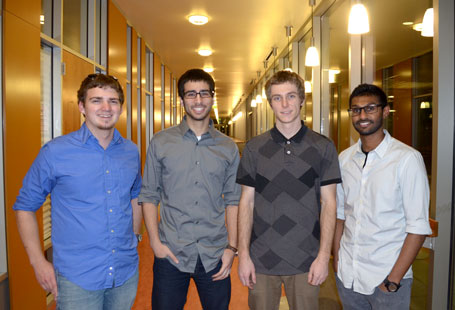
\includegraphics[width=0.42\textwidth]{al-group.jpg}}%
		}%
		%\\	% this spacer is needed to make the text on the right fit OK
	\end{wrapfigure}
	
	\NewsItem{Who Are We}
	\emph{We are a group of UC Santa Cruz computer and robotics engineering students who are building a robot to assist lifeguards in saving drowning individuals on beaches, at sea, and in other bodies of water. In the United States, there has been a reported 99 people that have drowned in the past year alone, with a good number of them occurring while a lifeguard was on duty. We propose an autonomous boat that can navigate to a person, allowing them to hang on and stay a float until the lifeguard arrives. Our aim is to keep beaches safer by reducing the risk of drowning.}
\end{minipage}
\end{center}
% -----


% 
% -----
\vspace{0.5cm}
	\SepRule
\vspace{0.5cm}
\begin{multicols}{3}
	\NewsItem{Progress}
	\NewsAuthor{D. Goodman}
    
    We are all very pleased to announce that our command center is nearing completion. As our school quarter comes to an end, our project continues to grow and progress. During March, many hours of our time was dedicated to implementing and integrating sensors, running GPS testing to 

    

	January has been a very productive month for our team. We are making substantial progress on the project. Throughout January, we have been hard at work writing, researching, coding, and soldering. Administratively, we have completed a Gantt chart, a website, and have entered into the Texas Instruments Analog Design Contest. In the hardware portion, we have purchased a boat and begun to modify it with new motors, electronic speed controllers, and batteries.  The command center---an encoded tripod assembly that the lifeguard will use to designate a drowning person---is coming together as well. We have acquired a tripod and absolute rotary encoders for triangulation. The encoder housing has been created, and a software interface is now in the works to take angular measurements and translate them into distance. Great care has been taken to ensure that the encoders are very precise so that we can triangulate the position of a drowning person accurately with minimal error. Many of our other sensors are nearly complete as well. We have an accelerometer up and running, our thermal imagining nearly complete, our altimeter is working, our GPSs running and we are analyzing their data in MATLAB, and we have been planning our approach to implementing the microwave radar and sonar sensors after inspecting their analog waveforms with an oscilloscope. 
\begin{center}
			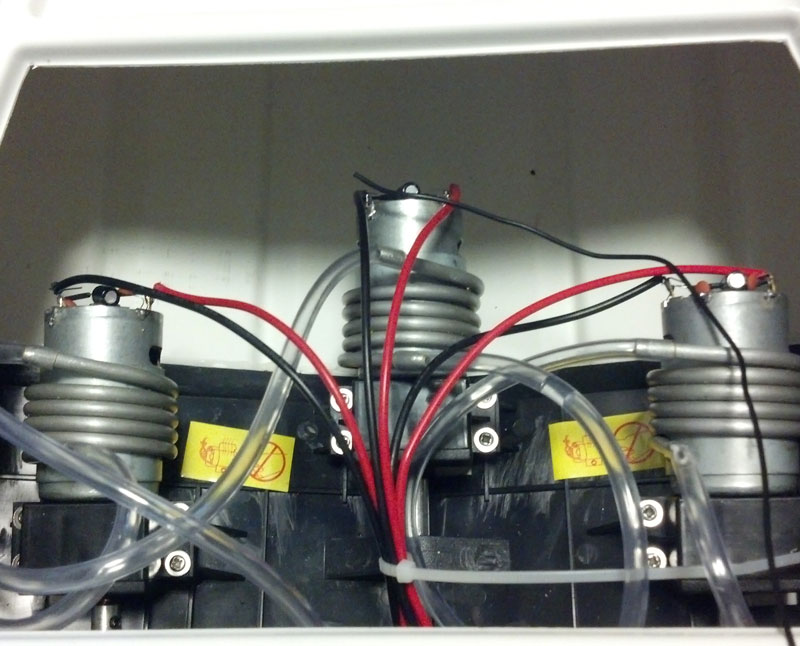
\includegraphics[width=0.78\linewidth]{old_motors.jpg}
		\end{center}
Overall, this past month has been productive on all fronts and the team is anxious to continue with work in February.
		
% -----

\vspace{1cm}
% Other news (2)
% -----
\NewsItem{Direction}
\NewsAuthor{D. Deo}
	Every week, the team specifies a minimum set of personal goals that they wish to complete.
 This week the group will focus on modeling accurate data from the encoders, XBee, GPS, and thermal sensor. The goal is to get the encoders to read accurate angles and have the ability to be calibrated to a zero degree point within software. Data from the GPS and XBee need to be obtained over a duration of time to analyze and correct for any error that may be present. The thermal sensor data is to be mapped to an RGB array so that heat signatures may be seen in real time. These sensors and modules are the last that need be implemented before the integration phase where the various components will be mounted on their respective subsystem. Comprehensive testing will occur after each sensor is up and running. We will also begin designing hierarchical finite state machines for the boat and the command center. These will provide our systems with the intelligence to act autonomously and make decisions on its own. So far, we are ahead of schedule for February.

% -----
%\columnbreak
\vspace{1cm}
% Other news (2)
% -----
\NewsItem{Support}
\NewsAuthor{D. Deo}
The Autonomous Lifeguard Group is moving quite swiftly and is hopeful that the next phases of the project will yield exceptional results. As a devoted team, we are currently funding the project entirely ourselves. Optimistic about the future of the Autonomous Lifeguard Project, we would appreciate any form of support that would help the project advance. Donations are welcome and can be submitted via our website. All considerations will be recognized by the team.
\end{multicols}
% -----
\end{document} 

